\chapter{Propuesta de solución}\label{chapter:proposal}

Este capítulo introduce la propuesta desarrollada para enfrentar el reto de clasificar de manera automática el cáncer de piel, empleando técnicas de aprendizaje profundo. La solución se centra en la utilización de una red neuronal profunda pre-entrenada, combinada con un algoritmo propio para el ajuste de precisión.

En el núcleo de nuestra estrategia se encuentra el uso de una red neuronal convolucional pre-entrenada llamada \textit{EfficientNetB1}. Esta red, desarrollada a partir de extensos conjuntos de datos y experiencias previas, ofrece una base sólida y rica en características para nuestro modelo. Al aprovechar este pre-entrenamiento, podemos acelerar significativamente el proceso de aprendizaje del modelo, al tiempo que aumentamos su capacidad para generalizar y reconocer patrones complejos en las imágenes dermatoscópicas.

Para complementar nuestro enfoque metodológico, seleccionamos herramientas tecnológicas avanzadas. Estas herramientas están diseñadas para optimizar el rendimiento del modelo, mejorar la precisión de la clasificación y garantizar una implementación efectiva. Entre ellas, destaca una capa de normalización, una capa densa, una de regularización, una \textit{dropout} y una de salida (capa densa con activación \textit{softmax}). Estas técnicas permite al modelo afinar su capacidad de identificar con precisión las diferentes categorías de lesiones cutáneas.

Para la optimización del algoritmo además se llevaron a cabo una serie de experimentos de los que se detallan en esta sección los 2 más relevantes. Estos experimentos se realizaron con el objetivo de encontrar la mejor configuración de datos para el modelo, que permita obtener la mayor precisión posible. Para esto se utilizaron dos técnicas de normalización de datos: division asimétrica con utilización de pesos por clases y estratificación de datos. Además se generaron distintas distribuciones de datos para los diferentes acercamientos.

Con la intensión de evaluar la efectividad y precisión del modelo se utilizo el conjunto de datos mencionado en capítulos anteriores HAM1000. Este conjunto de datos, con más de 10000 imágenes, representa una variedad de condiciones de la piel, lo que lo convierte en un recurso valioso para entrenar y evaluar algoritmos de detección de cáncer de piel. Para esto se importan, modelan y dividen los datos para asegurar un aprendizaje efectivo

La sección que sigue detalla la metodología empleada en la preparación y carga de los datos. Esta fase es esencial, ya que la calidad y el tratamiento de los datos tienen un impacto directo en la eficacia del modelo.

\section{Preparación y carga de datos}

En la presente sección, se describe cómo se seleccionó y procesó el conjunto de datos HAM10000, una colección extensa y diversa de imágenes dermatoscópicas. Se comienza por el \textit{dataset} escogido para entrenamiento y validación y luego se profundiza en la transformación de los datos, detallando las técnicas aplicadas para optimizar el rendimiento del algoritmo. Esto incluye el procesamiento de las imágenes y la conversión de los metadatos a un formato categórico adecuado para su análisis.

Posteriormente, se explica la modelación y división del conjunto de datos, utilizando herramientas como Pandas para estructurar los datos y dividirlos en conjuntos de entrenamiento, validación y prueba. Finalmente, se aborda el desafío del desequilibrio en la representación de las clases dentro del \textit{dataset}. Se detallan las estrategias implementadas para equilibrar el conjunto de datos, garantizando así que el modelo aprenda de manera efectiva a identificar una variedad de lesiones cutáneas sin sesgos hacia las condiciones más comunes.

\subsection{Dataset}

El conjunto de datos HAM10000, acrónimo de \textit{Human Against Machine with 10000 training images} (Humano Contra Máquina con 10000 imágenes de entrenamiento), se presenta como una solución al problema de la falta de diversidad y tamaño reducido en los conjuntos de datos disponibles para el diagnóstico automatizado de lesiones cutáneas pigmentadas. Este conjunto de datos es notable por su extenso alcance y diversidad, abarcando una amplia gama de lesiones cutáneas pigmentadas comunes \brackcite{tschandl2018ham10000}. 

\subsubsection*{HAM10000}

Las $10015$ imágenes dermatoscópicas del conjunto de datos HAM10000 se recopilaron a lo largo de 20 años desde dos ubicaciones diferentes: el Departamento de Dermatología de la Universidad Médica de Viena, Austria, y la práctica de cáncer de piel de Cliff Rosendahl en Queensland, Australia {tschandl2018ham10000}. En comparación con otros conjuntos de datos, HAM10000 ofrece un conjunto más diverso y completo de imágenes dermatoscópicas para la investigación del aprendizaje automático. Las imágenes y los metadatos del HAM10000 están disponibles públicamente a través del archivo ISIC \brackcite{tschandl2018ham10000} tienen la siguiente distribución.

\begin{table}[ht]
   \centering
   \begin{tabular}{lccc}
   \hline
   \textbf{Categoría Diagnóstica} & \textbf{Número de Imágenes} & \textbf{Porcentaje} \\
   \hline
   Melanocytic nevi               & 6705                        & 66.95\%             \\
   Melanoma                       & 1113                        & 11.11\%             \\
   Benign keratosis-like lesions  & 1099                        & 10.97\%             \\
   Basal cell carcinoma           & 514                         & 5.13\%              \\
   Actinic keratoses              & 327                         & 3.27\%              \\
   Vascular lesions               & 142                         & 1.42\%              \\
   Dermatofibroma                 & 115                         & 1.15\%              \\
   \hline
   \end{tabular}
   \caption{Distribución de imágenes por categoría diagnóstica}
   \label{tab:ham10000_distribution}
\end{table}   
   
Las imágenes almacenadas, originalmente como diapositivas, fueron digitalizadas usando un escáner \textit{Nikon Coolscan 5000 ED}. Posteriormente, se ajustaron manualmente para centrar las lesiones y se aplicaron correcciones al histograma para mejorar el contraste visual y la reproducción del color. Para separar eficientemente las imágenes dermatoscópicas de otros tipos de imágenes (como primeros planos y vistas generales), se utilizó un método automatizado que clasificaba más de 30,000 imágenes. Se empleó una arquitectura \textit{InceptionV3}, entrenada con un conjunto de imágenes etiquetadas manualmente, para categorizar las imágenes. Las imágenes mal clasificadas por este método fueron revisadas y corregidas manualmente.  Se realizó una revisión manual final para excluir imágenes con ciertos atributos no deseados, como contenido potencialmente identificable, imágenes fuera de enfoque o con artefactos perturbadores como prendas, y lesiones completamente no pigmentadas. Las imágenes restantes fueron revisadas para asegurar una reproducción de color y luminosidad adecuadas, aplicando correcciones manuales si era necesario \brackcite{tschandl2018ham10000}. 


Los datos utilizados como medio de aprendizaje para este proyecto son imágenes y metadatos. El dataset HAM10000 contiene imágenes tomadas de varios tipos de cáncer de piel y un archivo de metadatos que contienen información relacionada con cada imagen en formato \textit{one hot encoding}. Esta una técnica de procesamiento de datos en la cual cada valor categórico se representa mediante un vector binario cuyo tamaño corresponde al número de categorías posibles. En dicho vector, todos los elementos son cero, salvo el correspondiente a la categoría del valor, que es uno \brackcite{ohe}. 

\subsection{Transformación de datos}

Los metadatos asociados a la clasificación, etiquetados con método mencionado (\textit{one hot encoding}), fueron convertidos a un formato \textit{categórico} \brackcite{vitalflux_categorical_crossentropy} para su procesamiento. En este proceso a cada elemento se le asignan etiquetas a las basándose en las categorías de lesiones cutáneas, como 'MEL' (Melanoma), 'NV' (Nevus Melanocítico), entre otras. Se elimina del \textit{dataframe} además cualquier columna innecesaria, dejando solo las etiquetas y nombres de imágenes relevantes. De tal forma que los datos quedan distribuidos por clase.

\begin{table}[ht]
   \centering
   \begin{tabular}{lccc}
   \hline
   \textbf{index} & \textbf{Imágenes} & \textbf{Etiqueta} \\
   \hline
      0 & $ISIC\_0024306.jpg$ & NV \\
      1 & $ISIC\_0024307.jpg$ & NV \\
      2 & $ISIC\_0024308.jpg$ & NV \\
      3 & $ISIC\_0024309.jpg$ & NV \\
      4 & $ISIC\_0024310.jpg$ & MEL \\
   \hline
   \end{tabular}
   \caption{Datos transformados a formato categórico}
   \label{}
\end{table}   

\subsection{Modelación y división del conjunto de datos}

Los datos se modelan a partir de un \textit{dataframe} de Pandas \brackcite{pandas}. Estos son divididos en 3 conjuntos: Entrenamiento, Validación y Prueba, utilizando un enfoque simple de division de datos en porcentaje. Estas divisiones son necesarias para que el modelo pueda aprender y ser evaluado correctamente.

Inicialmente, el conjunto de datos, fue dividido en dos subconjuntos: \textit{train}, que se destinó para el entrenamiento, y \textit{dummy}, que fue utilizado como una combinación temporal para los conjuntos de validación y prueba. Luego el segundo conjunto fue separado en \textit{valid}, destinado a la validación y \textit{test}, utilizado para las pruebas.

\subsection{Generadores de datos y preprocesamiento}

Uno de los principales problemas del dataset, como se puede observar en la tabla 2.1, es el desequilibrio en la representación de las clases, un problema habitual en los conjuntos de datos médicos en los que algunas enfermedades son más raras que otras. Para solucionar este problema, el conjunto de datos se equilibra meticulosamente limitando el número máximo de muestras por clase. Esto garantiza que el modelo no esté sesgado hacia las clases más comunes y pueda generalizar mejor entre varios tipos de lesiones cutáneas. 

En cada experimento, la cantidad de muestras por clase se ajustó de manera selectiva. Por ejemplo, en el experimento 1 se utilizaron 300 muestras por clase, mientras que en el experimento 2 se incrementó a 500 muestras. Incluso en el subconjunto de 300 muestras, algunas clases contaban con menos de 300 ejemplos, lo que llevó a la implementación de la técnica de \textit{class weighting} \brackcite{analyticsvidhya2020classweight}. Este método asigna pesos diferenciados a cada clase durante el entrenamiento del modelo, reforzando así la señal de aprendizaje para las clases menos representadas.

Además, a los conjuntos segmentados en entrenamiento, validación y prueba, se les aplicó \textit{data augmentation}. Esta técnica incluye varias transformaciones a las imágenes, como rotación, desplazamiento y zoom, durante su carga, generando lotes de imágenes optimizados para el entrenamiento y evaluación del modelo \brackcite{augmentation}.

\section{Desarrollo del modelo y estrategias de optimización}\label{sec:method}
%-----------------------------------------------------------------------------------

\subsection{Selección del modelo y transferencia de aprendizaje}

Para abordar efectivamente el desafío de la detección de cáncer de piel, se seleccionó la arquitectura \textit{EfficientNetB1} \brackcite{efficientnet} como base del modelo. Esta red neuronal convolucional, parte de la familia EfficientNet, se caracteriza por su alta eficiencia y precisión. Utilizando un modelo pre-entrenado, se aprovechan los pesos derivados de conjuntos de datos extensos, lo que facilita la adaptación del modelo a nuestro conjunto de datos específico, el HAM10000 \brackcite{tan2019efficientnet}.

\subsection{Diseño y entrenamiento del modelo}

El modelo \textit{EfficientNetB1} se carga pre-entrenado con pesos de \textit{ImageNet} \brackcite{Pinecone2021ImageNet}, una amplia base de datos de imágenes ampliamente utilizada para entrenamiento y \textit{benchmarking} en visión por computadora. Al omitir la capa superior del modelo, se permite la incorporación y personalización de capas adicionales. La salida del modelo base se somete a una serie de transformaciones, incluyendo normalización por lotes, capas densas con regularizaciones, y técnicas de \textit{Dropout} para prevenir el sobre-ajuste, culminando en una capa de salida optimizada para la clasificación.

\subsection{Arquitectura del modelo EfficientNet}
   
La familia de arquitecturas EfficientNet, desarrollada por los autores en \brackcite{tan2019efficientnet}, surgió con el objetivo de hallar un método adecuado para escalar las CNNs de manera que mejoraran tanto en precisión (i.e., rendimiento del modelo) como en eficiencia (es decir, en términos de parámetros del modelo y FLOPS). Estos autores propusieron un método de escalado compuesto que utiliza un conjunto fijo de coeficientes para escalar de manera uniforme el ancho, la profundidad y la resolución de la red. El método les permitió desarrollar una arquitectura de CNN eficiente, a la que denominaron EfficientNet B0. Posteriormente, crearon las variantes EfficientNets B1-B7 escalando la red base (EfficientNet B0).
   
Mientras que la arquitectura EfficientNet B0 tiene $5.3$ millones de parámetros y acepta imágenes de entrada de $224x224$, EfficientNet B7 cuenta con $66$ millones de parámetros y acepta imágenes de $600x600$ \brackcite{Tan2019EfficientNetRM}.
   
   \begin{figure}[ht]%
      \begin{center}
      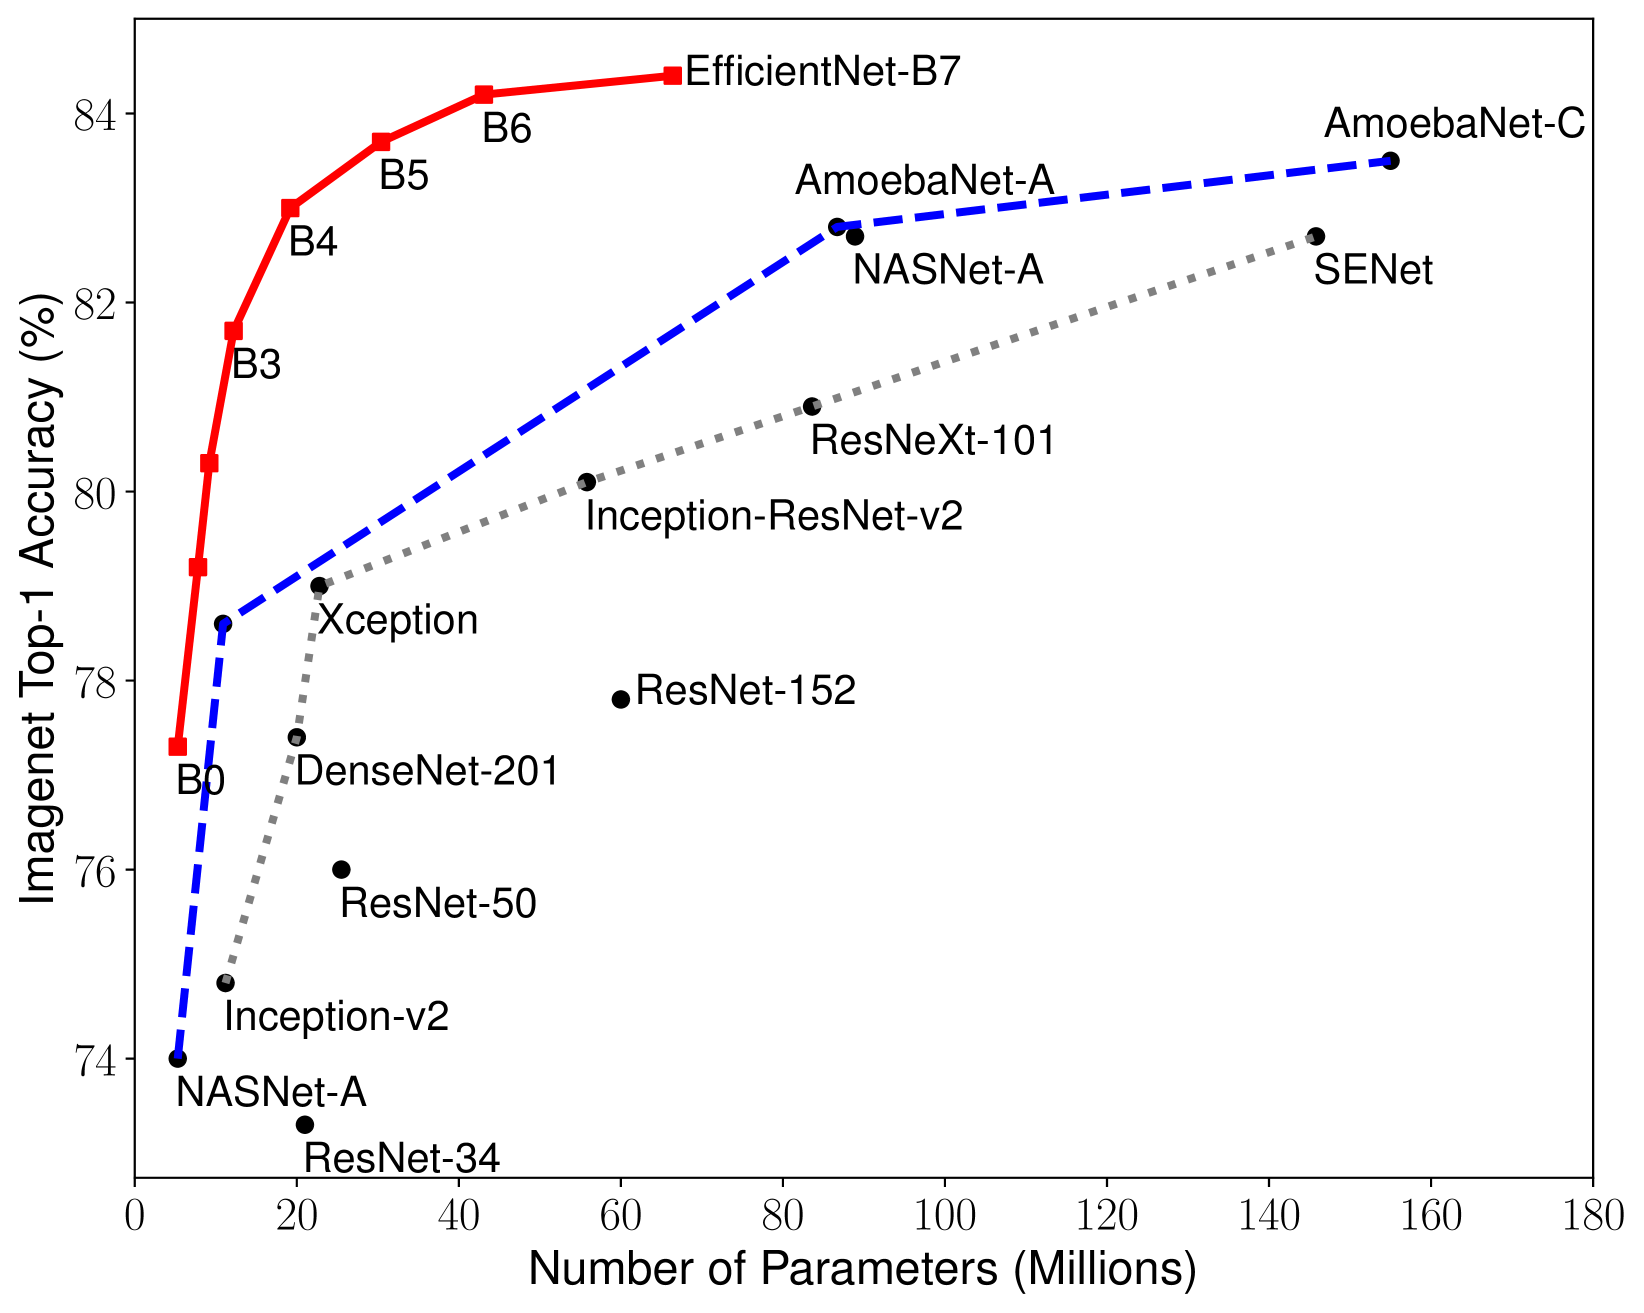
\includegraphics[width=1\textwidth]{./Graphics/efficientnet_performance.png}
      \caption{Estadísticas del rendimiento de los modelos de EfficientNet}
      \label{fig:efficientnet_performance}
      \end{center}
      \end{figure}
   
\subsection{EfficientNetB1}
   
   En relación con el dataset HAM1000 \brackcite{ham10000}, la implementación del EfficientNetB1 puede ser particularmente beneficiosa para el análisis de datos. EfficientNetB1, entre las variantes de la serie EfficientNet, se encuentra en un punto medio en términos de complejidad y tamaño, ofreciendo un equilibrio entre precisión y eficiencia computacional. Dado que el HAM1000 es un conjunto de datos de imágenes dermatoscópicas que requiere una alta precisión en la identificación y clasificación de lesiones cutáneas, la utilización de EfficientNetB1 podría proporcionar una precisión y eficiencia aceptable en términos de recursos computacionales.

\subsection{Arquitectura del Modelo y Regularización}

Para fortalecer la arquitectura del modelo, se añadieron capas adicionales, incluyendo Dropout y regularizadores L1 y L2, esenciales para combatir el sobre-ajuste. Una capa densa personalizada fue incorporada para facilitar la clasificación precisa de múltiples tipos de tumores. La compilación del modelo se realizó con un enfoque en la clasificación multi-clase, utilizando la pérdida de entropía cruzada categórica y un optimizador adecuado, seleccionados por su efectividad en tareas similares.

\subsection{Ajuste dinámico del learning rate}

Un elemento innovador del entrenamiento fue la implementación de un callback personalizado para el ajuste dinámico del learning rate. Esta estrategia permite ajustes adaptativos del learning rate basados en el rendimiento del modelo, optimizando la eficiencia del entrenamiento y evitando el estancamiento en mínimos locales del espacio de búsqueda.


\section{Experimentos}

\subsection{Experimento 1: Evaluación de la eficiencia de la división asimétrica de datos en la clasificación de imágenes de cáncer de piel}

Este experimento se centra en una división de datos altamente asimétrica, con un enfoque predominante en el conjunto de entrenamiento. La técnica de \textit{dummy split} se emplea para mantener proporciones consistentes entre los conjuntos de validación y prueba. Esta metodología es relevante para evaluar el impacto de un extenso conjunto de entrenamiento en la precisión y el rendimiento del modelo.

subsection{Experimento 2: Análisis de la estratificación de datos en la clasificación de imágenes de cáncer de piel}

Descripción: Este experimento explora la estratificación de datos para mantener una distribución uniforme de etiquetas en cada conjunto de datos. La proporción de los conjuntos de datos es más equilibrada en comparación con el Experimento 1, lo que ofrece insights sobre la importancia de la distribución equitativa de datos en el entrenamiento y evaluación de modelos.